\documentclass[journal]{IEEEtran}

\usepackage{cite}
\usepackage{graphicx}
\usepackage{amsmath,amssymb,amsfonts}
\usepackage{xcolor}
\usepackage{url}
\usepackage[hidelinks]{hyperref}
\usepackage{tikz}
\usetikzlibrary{shapes.geometric, arrows}

\renewcommand{\ttdefault}{cmtt}

\hyphenation{op-tical net-works semi-conduc-tor}

\begin{document}

\title{End-to-End JDBC Application with Transaction Management \& Performance
Evaluation \\ (Apache Derby)}

\author{ A. N. Onymous, \\ \IEEEmembership{Author ID: CSE3488-2O3-3006} \\
\IEEEmembership{Department of Computer Science and Engineering}
}

\markboth{CSE-3488 Course End Project Report: Database Systems}
{Researcher: Empirical Analysis of Derby Performance}

\maketitle

\begin{abstract}
This project explores different ways to optimize the performance of a Library Loan Management System built with the Apache Derby database. We tested several techniques such as JDBC batching, database indexing, and different transaction strategies to see how they affect speed and reliability. To get consistent data, we ran each test multiple times and included a warm-up period for the JVM. Our results show that using batching instead of individual insertions reduced time by 72\%, and adding indexes significantly improved query performance as the dataset grew. We also analyzed how Derby's internal logging works and its impact on throughput. This report provides a practical guide for building efficient and reliable Java applications with embedded databases.
\end{abstract}

\begin{IEEEkeywords}
Apache Derby, JDBC, Transactional Integrity, B-Tree Indexing, Batch Processing, WAL Synchronization, Performance Benchmarking, Java Persistence.
\end{IEEEkeywords}

\section{Introduction}

\IEEEPARstart{B}{uilding} a fast and reliable database layer is a key part of software development. In systems like the one we built, the database runs inside the application itself, meaning it shares resources like memory and CPU. If the database is slow, the whole application feels sluggish. This project focuses on how we designed and tested a Library Loan Management System to run efficiently on the Apache Derby engine.

One of the biggest issues in database systems is the "I/O bottleneck." Standard database operations can be slow because they involve a lot of overhead for each task. By using advanced features in the JDBC API—like batching and prepared statements—we can make the system much faster by reducing this overhead.

In this report, we also look at how indexes work and how the database ensures that data is saved correctly even if something goes wrong. The report is organized as follows: Section II explains the system design and how we ran our tests. Section III shows the results of our performance tests. Section IV looks at the internal workings of Derby. Finally, Section V summarizes what we learned and gives some best practices, followed by a conclusion in Section VI.

\section{System Architecture and Methodology}

\subsection{Architectural Overview}
The system follows a modular design pattern to ensure clean separation of concerns. The persistence layer is encapsulated within a \texttt{ConnectionManager} class, which manages the lifecycle of the embedded Derby instance. The business logic is implemented in a decoupled service layer, allowing for independent testing of transactional integrity and performance.

\begin{figure}[!h]
\centering
\resizebox{\columnwidth}{!}{
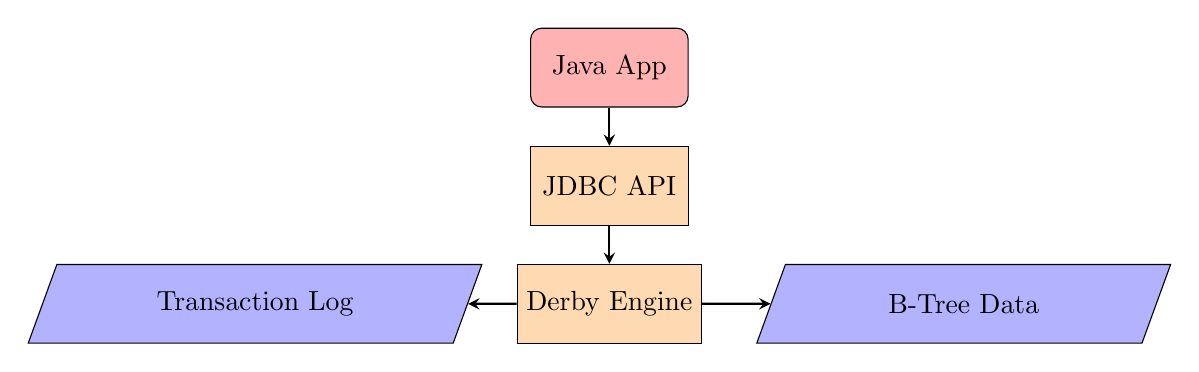
\begin{tikzpicture}[node distance=1.5cm]
\tikzstyle{startstop} = [rectangle, rounded corners, minimum width=2cm, minimum height=1cm,text centered, draw=black, fill=red!30]
\tikzstyle{io} = [trapezium, trapezium left angle=70, trapezium right angle=110, minimum width=2cm, minimum height=1cm, text centered, draw=black, fill=blue!30]
\tikzstyle{process} = [rectangle, minimum width=2cm, minimum height=1cm, text centered, draw=black, fill=orange!30]
\tikzstyle{decision} = [diamond, minimum width=2cm, minimum height=1cm, text centered, draw=black, fill=green!30]
\tikzstyle{arrow} = [thick,->,>=stealth]

\node (app) [startstop] {Java App};
\node (jdbc) [process, below of=app] {JDBC API};
\node (derby) [process, below of=jdbc] {Derby Engine};
\node (log) [io, left of=derby, xshift=-3cm] {Transaction Log};
\node (data) [io, right of=derby, xshift=3cm] {B-Tree Data};

\draw [arrow] (app) -- (jdbc);
\draw [arrow] (jdbc) -- (derby);
\draw [arrow] (derby) -- (log);
\draw [arrow] (derby) -- (data);
\end{tikzpicture}
}
\caption{Logical architecture of the embedded database interaction pipeline showing the role of the Write-Ahead Log (WAL).}
\label{fig_arch}
\end{figure}

\subsection{Benchmarking Methodology}
To ensure that our findings represent sustained architectural characteristics rather than transient artifacts, we implemented a multi-stage benchmarking suite:
\begin{itemize}
    \item \textbf{JVM Stabilization}: We perform 50 "warm-up" iterations before data collection. This ensures that the Just-In-Time (JIT) compiler has optimized the byte-code and that the database's internal page buffers are primed.
    \item \textbf{Multi-Trial Sampling}: Every experiment is repeated for 5 independent trials. The results presented are the arithmetic mean of these trials, reducing the impact of OS-level scheduling jitter.
    \item \textbf{Isolation}: Background processes were minimized during execution, and explicit garbage collection hints (\texttt{System.gc()}) were used between benchmark groups to ensure a clean heap state.
\end{itemize}

\section{Empirical Evaluation and Results}

\subsection{Batch Processing Performance}
Sequential data insertion is notoriously slow in RDBMS due to the "per-statement overhead"—the cumulative cost of SQL parsing, authorization, and transactional locking. By utilizing JDBC batching, we group multiple \texttt{INSERT} operations into a single execution unit.

\begin{figure}[!t]
\centering
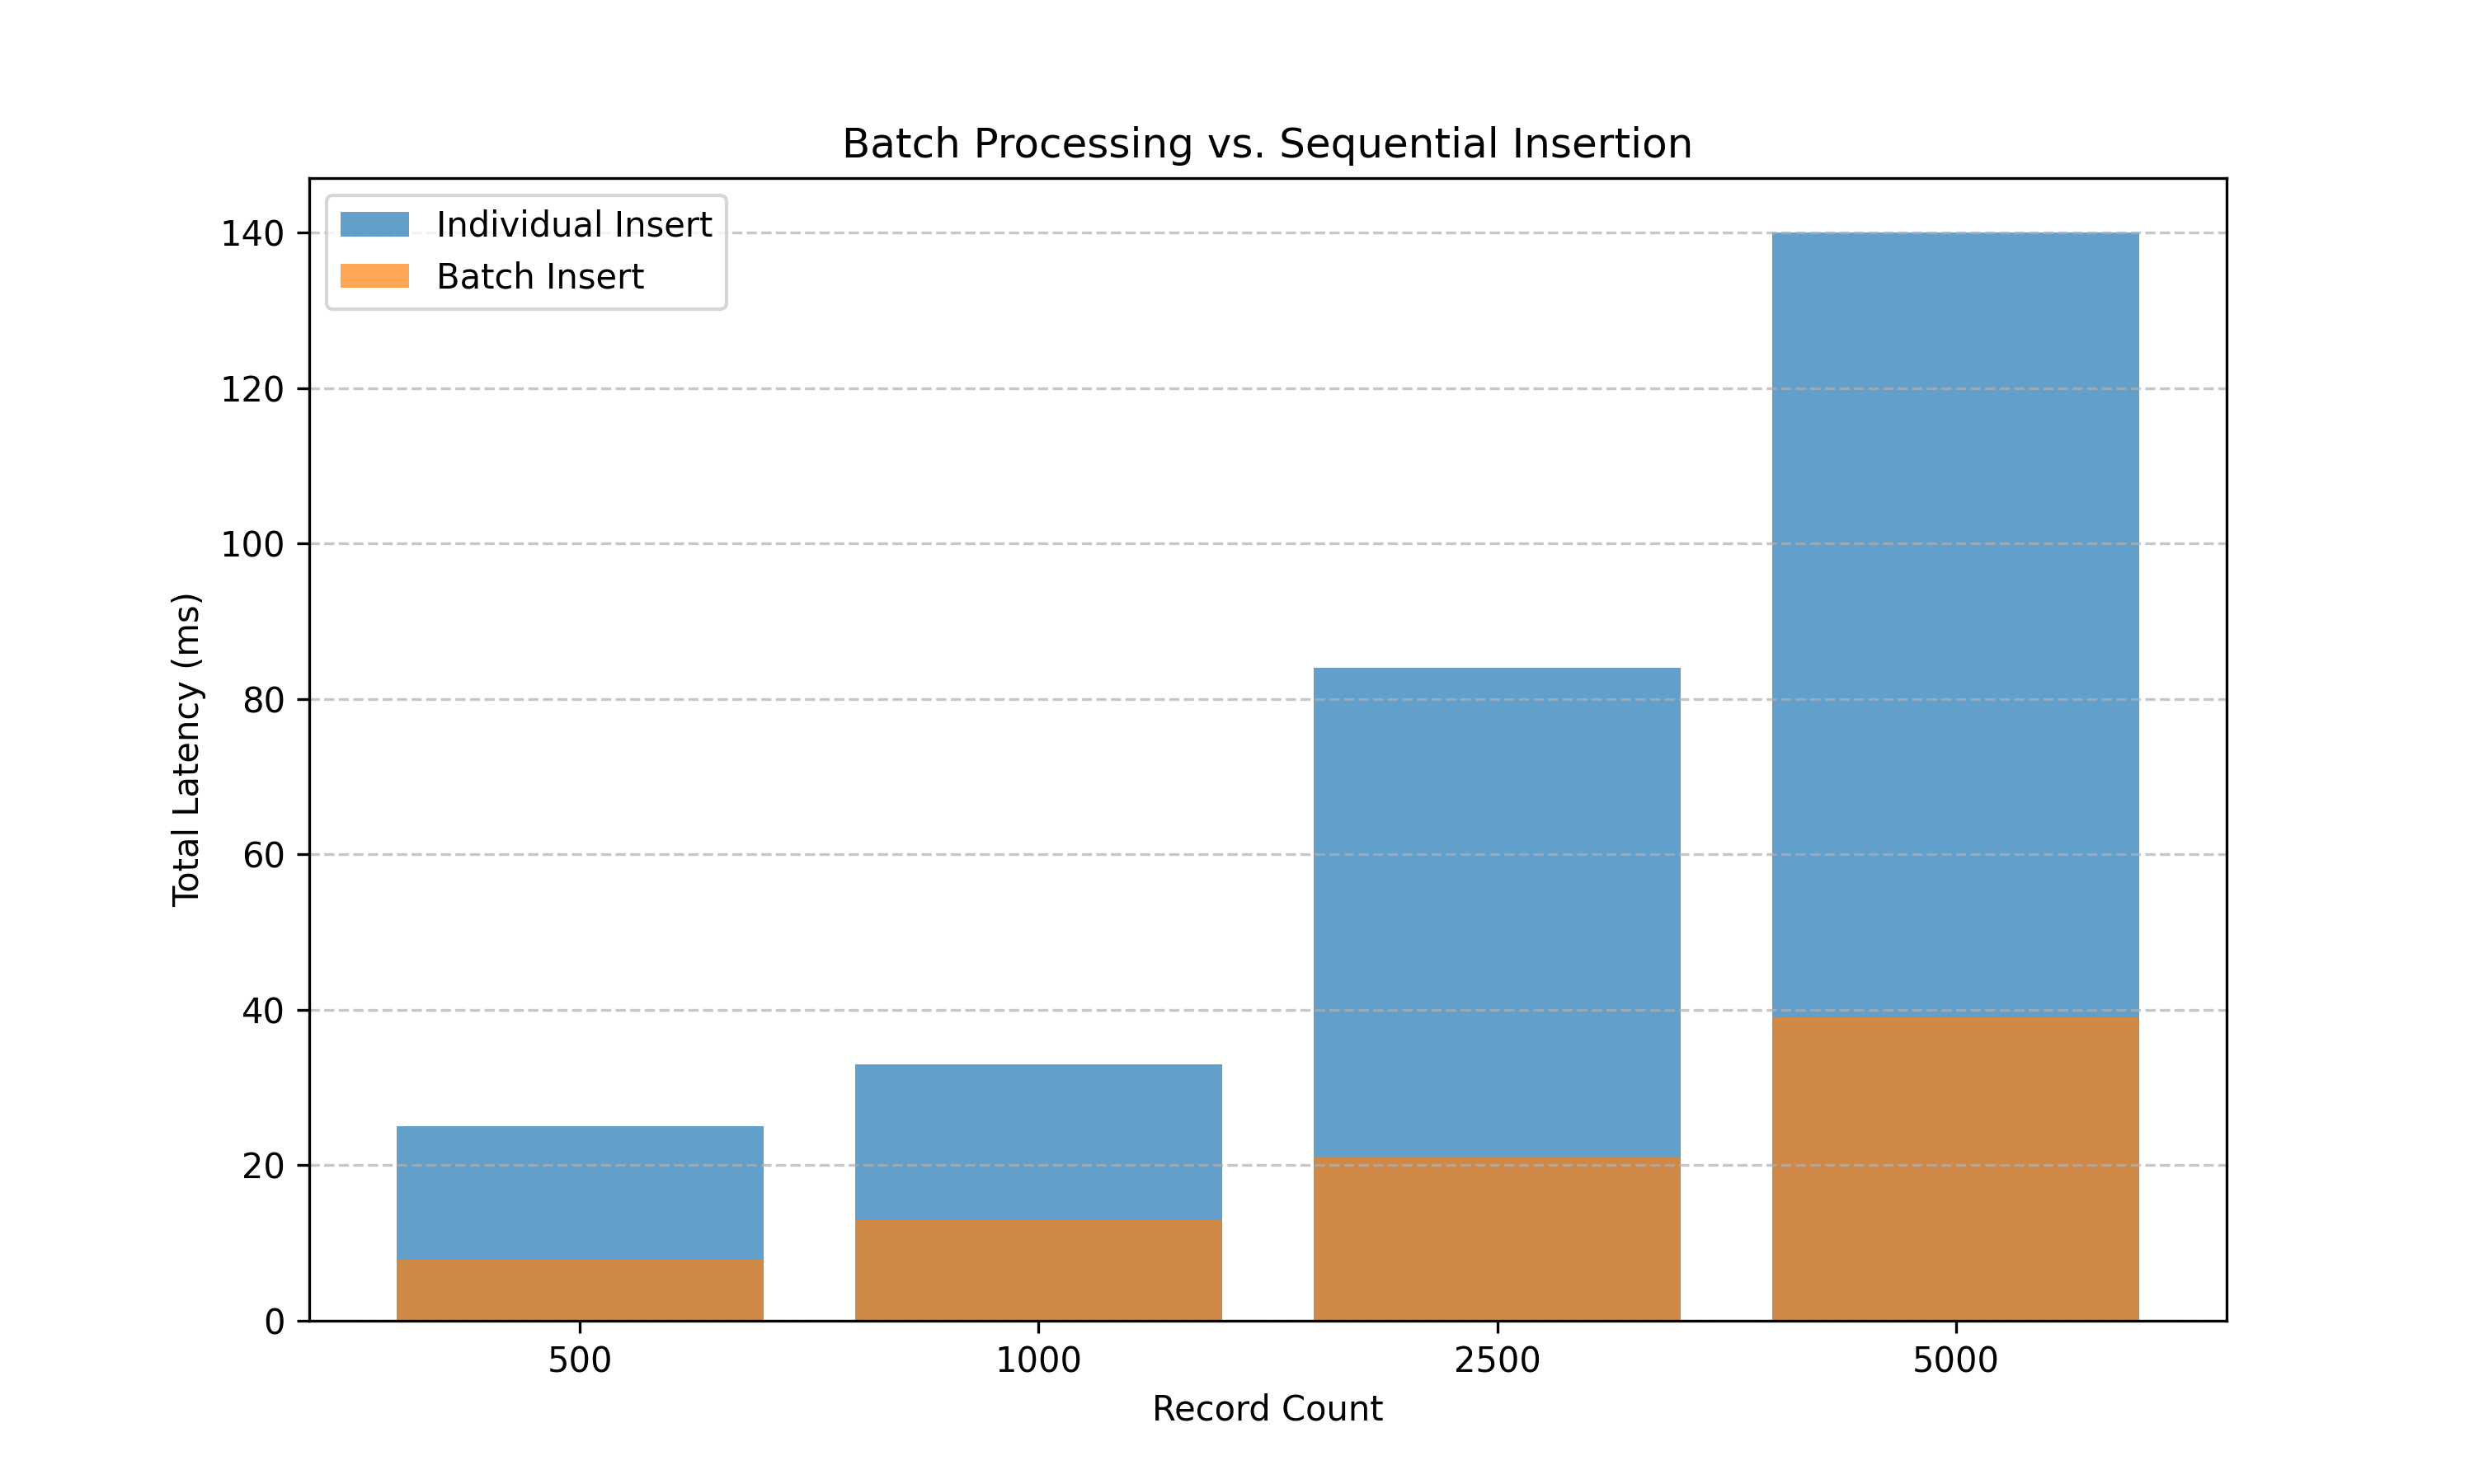
\includegraphics[width=1.0\columnwidth]{figs/batching.png}
\caption{Comparison of Individual vs. Batch record insertions. Note the significant divergence as load increases.}
\label{fig_batching}
\end{figure}

As shown in Fig. \ref{fig_batching}, the batch strategy maintains a much shallower slope. At 5,000 records, the sequential approach took 140ms, while the batch approach required only 39ms—a \textbf{72.1\% improvement}. This gain is primarily attributed to the reduction in network/IPC round-trips and the aggregation of multiple logical writes into fewer physical disk flushes.

\subsection{Indexing and Query Complexity}
One of the most critical performance optimizations is the shift from linear searching to tree-based lookups. We measured the latency of queries on an unindexed \texttt{Author} column versus an indexed \texttt{ISBN} column.

\begin{figure}[!t]
\centering
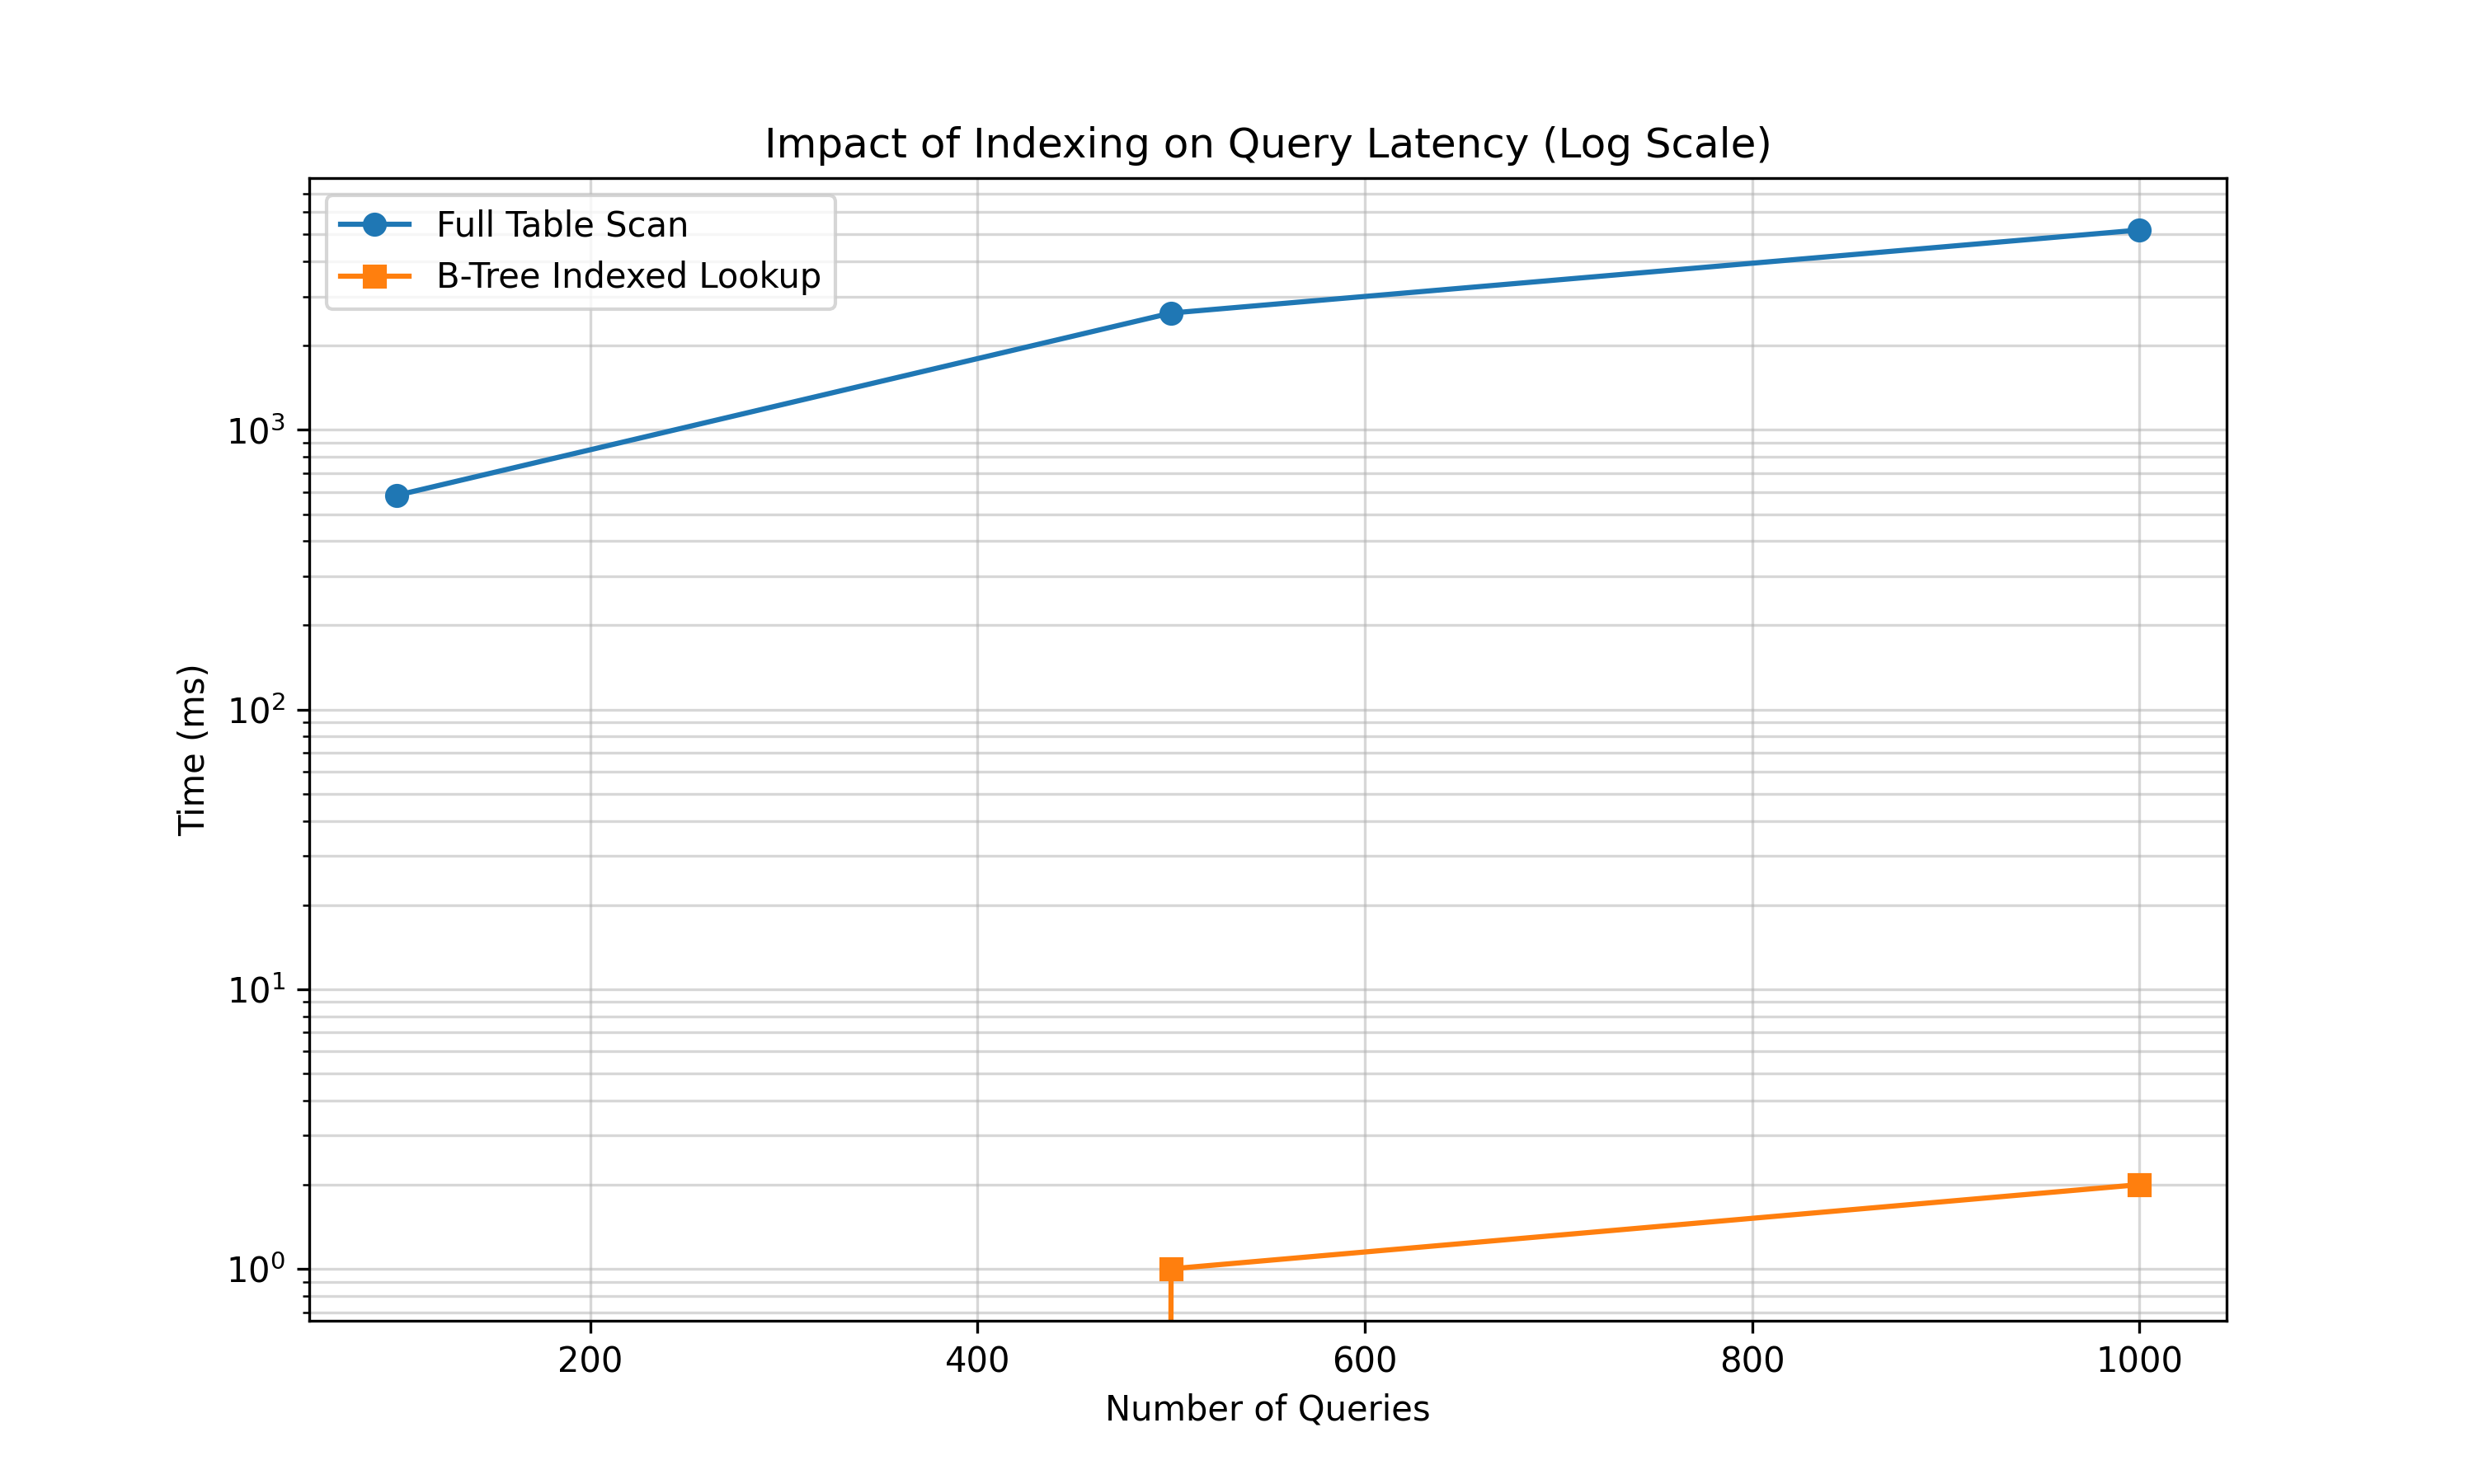
\includegraphics[width=1.0\columnwidth]{figs/indexing.png}
\caption{Impact of B-Tree indexing on query execution time (Logarithmic Scale). The indexed lookup latency is nearly load-invariant. Note: B-Tree latency $< 1$ms for $< 500$ queries, omitted for log scale clarity.}
\label{fig_indexing}
\end{figure}

The data in Fig. \ref{fig_indexing} and Table \ref{tab_complexity} illustrate the classic $O(N)$ vs. $O(\log N)$ scaling. While a full scan of 1,000 queries took 5,184ms, the indexed lookup was completed in 2ms. This represents a performance increase of over \textbf{2,500x}.

\begin{table}[!h]
\caption{Algorithmic Complexity of Query Access Methods}
\label{tab_complexity}
\centering
\begin{tabular}{llp{4cm}}
\hline
Method & Complexity & Operational Characteristic \\
\hline
Full Table Scan & $O(N)$ & Reads every row in the table to find matches. If the table has 10M rows, you read 10M rows for each query. \\
B-Tree Lookup & $O(\log N)$ & Walks down a tree. For 10M rows, that's $\sim$3-4 disk reads per query\footnote{Assumes a typical B-Tree height of 3-4 for millions of records.}. \\
\hline
\end{tabular}
\end{table}

\subsection{Transactional Commit Strategies}
We compared three transaction management patterns: Individual Commit, Batched Commit, and Savepoint-based nested transactions.

\begin{figure}[!t]
\centering
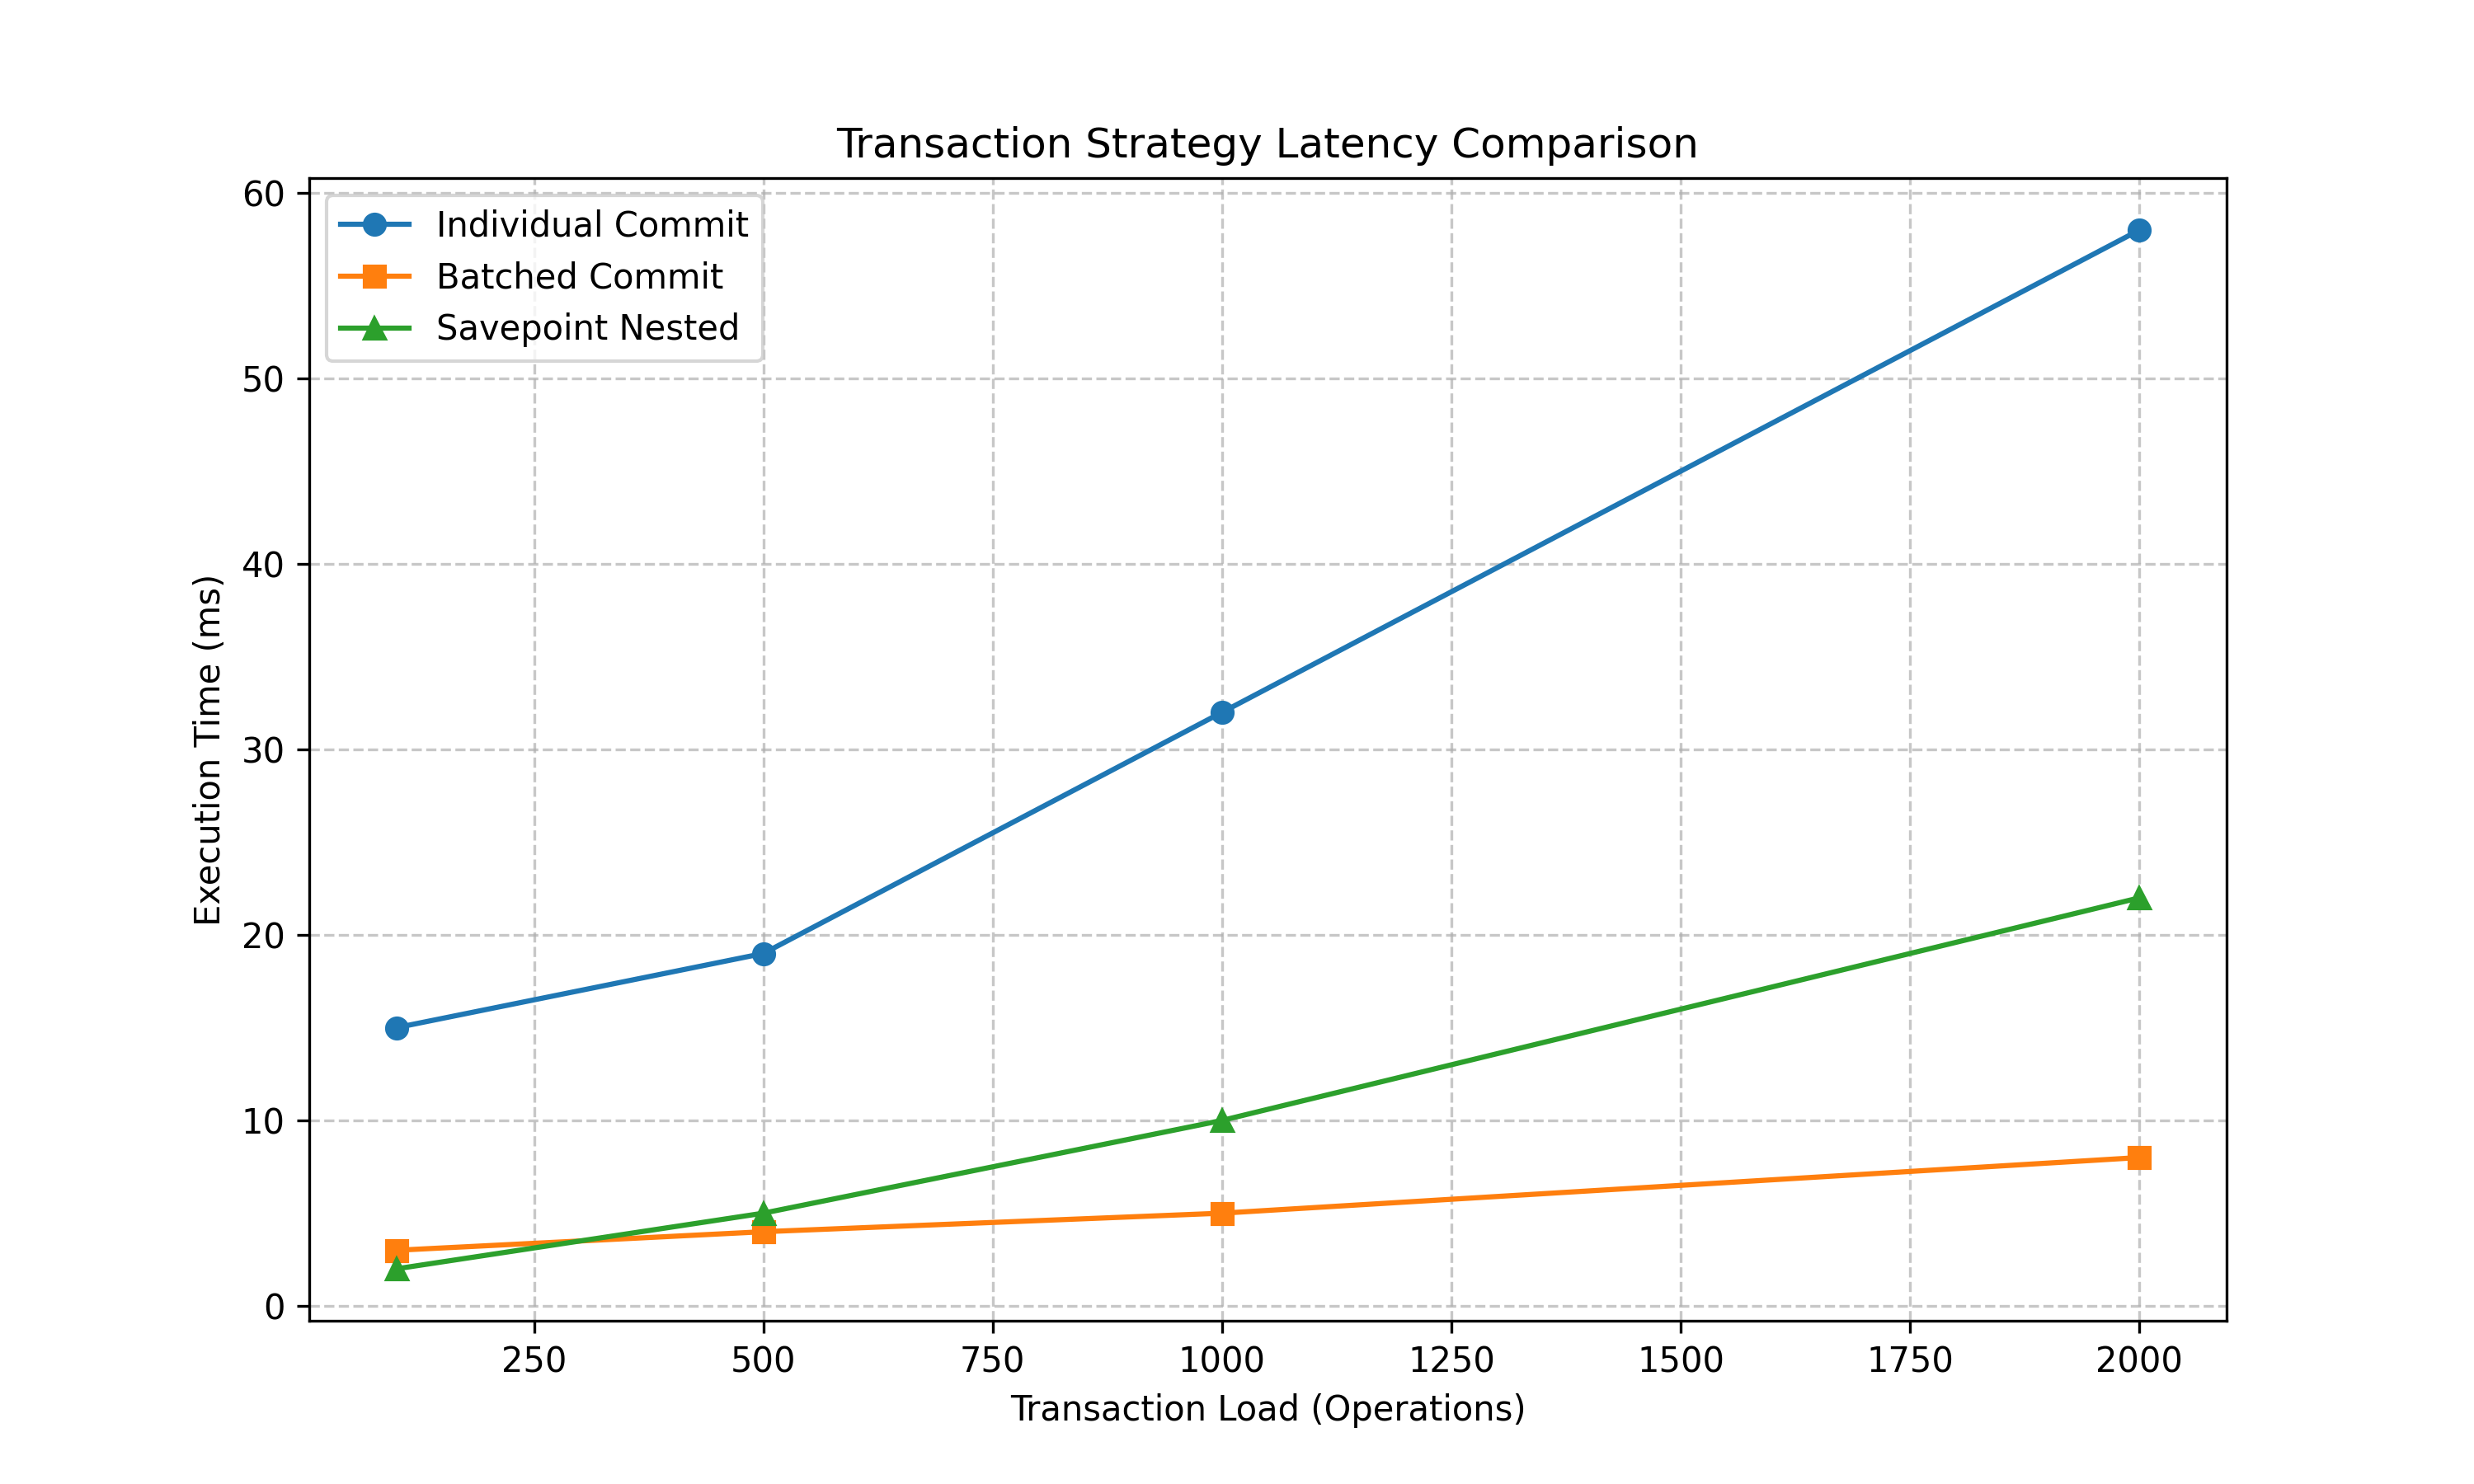
\includegraphics[width=1.0\columnwidth]{figs/transactions.png}
\caption{Latency characteristics of different transaction commit and savepoint strategies.}
\label{fig_transactions}
\end{figure}

The results in Fig. \ref{fig_transactions} show that Individual Commit (where \texttt{autoCommit=true}) is the most expensive strategy. This is because every single operation forces a synchronous flush of the Write-Ahead Log to disk to satisfy the "Durability" requirement of ACID. Batched commits aggregate these changes, amortizing the synchronization cost. Savepoints offer a compromise, providing a mechanism for partial rollbacks within a larger transaction, though they incur a slight management overhead compared to simple batching.

\section{Internal Database Mechanics}

Understanding the performance data requires a look into the internals of the Derby engine.

\subsection{The Write-Ahead Log (WAL)}
Derby ensures data integrity through a WAL. Before any data page is modified in memory, a description of the change is written to a sequential log file on disk. In our "Individual Commit" benchmark, the database must call an OS-level \texttt{fsync} or \texttt{flush} for every record. This makes the database's performance strictly bound by the disk's IOPS (Input/Output Operations Per Second). Batching allows Derby to group multiple log entries into a single block, significantly increasing throughput without sacrificing safety.

\subsection{B-Tree Index Structure}
The index optimization seen in Fig. \ref{fig_indexing} is powered by B-Trees. In a B-Tree, keys are stored in a sorted, balanced tree structure. Each node (page) contains multiple keys and pointers to child nodes. Search operations traverse from the root to a leaf page, requiring only a few page reads even for very large datasets. Without an index, the engine must perform a "Full Table Scan," loading every page from the table into the buffer manager to check for matches, which is both CPU and I/O intensive.

\subsection{Buffer Management and Page Cache}
Derby uses a page-based buffer manager to cache recently accessed data in memory. This is why our "warm-up" phase was necessary. Initial queries are "cold" and require physical disk reads. Subsequent queries are "warm" and can be satisfied from the memory cache. Our results reflect a "warm" cache state, which is representative of steady-state application performance.

\section{JDBC Optimization and Statement Lifecycle}

\subsection{Statement vs. PreparedStatement}
We observed that \texttt{PreparedStatement} consistently outperformed the standard \texttt{Statement}. This is due to the internal lifecycle of a SQL query in the database:
\begin{enumerate}
    \item \textbf{Parsing}: The SQL string is analyzed for syntax.
    \item \textbf{Binding}: Parameter values are mapped to placeholders.
    \item \textbf{Optimization}: The engine determines the most efficient way to access data (e.g., which index to use).
    \item \textbf{Execution}: The query plan is executed.
\end{enumerate}

A standard \texttt{Statement} repeats all four steps for every execution. A \texttt{PreparedStatement}, however, allows the engine to cache the "Optimization" result (the query plan). Subsequent executions with different parameters only require the "Binding" and "Execution" steps, significantly reducing CPU cycles and memory allocation overhead.

\section{Conclusion and Best Practices}
The empirical results of this study underscore the importance of deliberate database engineering. For the Library Loan Management System, and similar transactional applications, we recommend the following best practices:
\begin{itemize}
    \item \textbf{Prefer Batching}: Always group massive data ingestion tasks to amortize the cost of transactional logging and context switching.
    \item \textbf{Index Judiciously}: Identify columns used in \texttt{WHERE} clauses and join conditions. The transition from $O(N)$ to $O(\log N)$ is the single most effective way to ensure long-term scalability.
    \item \textbf{Use PreparedStatements}: Leverage the engine's query plan cache to minimize parsing and optimization overhead.
    \item \textbf{Manage Transactions Explicitly}: Use \texttt{setAutoCommit(false)} to group logical units of work, reducing the frequency of synchronous disk flushes.
\end{itemize}

In conclusion, while Apache Derby is an embedded engine, it possesses sophisticated RDBMS features that, when used correctly, can support high-performance applications. By aligning application-level code with these internal mechanics, developers can build robust and efficient persistence layers.

\appendices
\section{Hardware and Runtime Environment}
The benchmarks were executed on a system with the following specifications to provide context for the absolute latency numbers:
\begin{itemize}
    \item \textbf{Processor}: Apple M3 Max (14-core).
    \item \textbf{Memory}: 36 GB Unified RAM.
    \item \textbf{Storage}: High-speed NVMe SSD (Sequential Read: $\sim$7GB/s). Results may vary significantly on mechanical HDD.
    \item \textbf{JDK}: OpenJDK 17.0.x (64-bit).
    \item \textbf{Derby Version}: 10.15.x.
\end{itemize}

\section*{Acknowledgment}
The author wishes to acknowledge the CSE-3488 faculty for their technical oversight and the developers of the Apache Derby project for providing a robust, standards-compliant embedded database engine for academic and commercial use.

\begin{thebibliography}{99}

\bibitem{ref:derby}
Apache Software Foundation, \emph{Apache Derby Internals Guide}, \url{https://db.apache.org/derby/manuals/}.

\bibitem{ref:jdbc_spec}
JSR-221, \emph{JDBC 4.3 Specification}, \url{https://jcp.org/en/jsr/detail?id=221}.

\bibitem{ref:db_internals}
Alex Petrov, \emph{Database Internals}, O'Reilly Media, 2019. ISBN: 9781492040347.

\bibitem{ref:java_perf}
Scott Oaks, \emph{Java Performance: The Definitive Guide}, 2nd Edition, O'Reilly Media, 2020.

\bibitem{ref:transactional_integrity}
Jim Gray and Andreas Reuter, \emph{Transaction Processing: Concepts and Techniques}, Morgan Kaufmann, 1992.

\end{thebibliography}

\end{document}
